\documentclass[12pt, letterpaper]{article}
\usepackage[margin={1.5in}]{geometry}

\usepackage{amsmath}
\usepackage{amsthm}
\usepackage{amssymb}
\usepackage{amsfonts}

\usepackage{hyperref}
\usepackage{authblk}
\usepackage[acronym]{glossaries}
\usepackage{xcolor}
\usepackage{graphicx}

\hypersetup{
	colorlinks,
	linkcolor={red!50!black},
	citecolor={blue!50!black},
	urlcolor={blue!80!black}
}


% My commands
\newcommand{\R}{\mathbb{R}}
\newcommand{\N}{\mathbb{N}}
\newcommand{\Z}{\mathbb{Z}}
\newcommand{\T}{\mathrm{T}}
\newcommand{\E}{\mathbb{E}}
\newcommand{\Var}{\mathrm{Var}}
\newcommand{\Cov}{\mathrm{Cov}}
\newcommand{\Dcal}{\mathcal{D}}

\newtheorem{proposition}{Proposition}
\newtheorem{theorem}{Theorem}
\newtheorem{example}{Example}

\makeglossaries
\newacronym{dro}{DRO}{Distributionally Robust Optimization}
\newacronym{dddro}{DDDRO}{Decision-Dependent Distributionally Robust Optimization}
\newacronym{flp}{FLP}{Facility Location Problem}

\title{
	Decision-Dependant Distributionally Robust Optimization \\
	\large Facility Location Problem with Random Demands
}
\author[1]{Gabriel Fortin-Leblanc}
\author[2]{Mohammad Joshaghani}
\affil[1]{Université de Montréal}
\affil[2]{Université du Québec à Montréal}
\date{December 15, 2024}

% Requested:
% [ ] 15-20 pages
% [x] Presentation of the decision problem in its deterministic form
% [x] Motivation regarding the key uncertainties in this problem
% [x] Presentation of a robust optimization model
% [ ] Short review of closely related litterature
% [ ] Description of the solution scheme (either through reformulation or decomposition methods)
% [ ] Presentation of experimental setup
% [ ] Summary of numerical findings
% [ ] Improvements?
% [ ] Add an abstract?

\begin{document}
	\maketitle
	\tableofcontents
	\newpage
	
	\section*{Introduction}
	Facility location is an important problem in transportation and logistics systems. It involves decisions about where to establish facilities to serve customer demands effectively while minimizing costs \cite{cornuejols_uncapicitated_1983}. Traditionally, facility location models assume demand is exogenous, fixed, or governed by a known probability distribution, but the models became more complex to better reflect reality. It has been used for multiple tasks that go further than positioning ``facilities", like positioning fire departments and their vehicles \cite{rodriguez_simulation-optimization_2021}, or even positioning testing facilities for COVID-19 \cite{liu_testing_2023}. The current monograph presents the facility location problem when demand is a random variable over a finite support \cite{basciftci_distributionally_2021}. 
	
	Consider the problem with $J$ customer sites and $I$ possible location for new facilities. The decision variable is $y \in \{0, 1\}^I$ where for some $i \in [I]$, $y_i = 1$ represents the decision of opening the facility at the location assigned to the index $i$ or not opening the facility if $y_i = 0$. Moreover, other information on those possible sites are available: $O \in \R_+^I$ the opening costs, $C \in \R_+^I$ the capacities and $t \in \R_+^{I \times J}$ the transportation fees for transporting one unit of merchandise from a facility to a customer site. About those lasts, $r \in \R_+^J$ the revenue for selling one item and $\Dcal = \{\xi_k \in \R_+: k \in [K]\} \subset \R_+^K$ the support for the demand are known. To simplify the notation suppose that $\xi_k < \xi_{k+1}$ for any $k \in [K-1]$ and denote $D = \max \Dcal$. Note that the support of the demand is the same for every customer sites. The deterministic model is
	\begin{subequations} \label{eq:deterministic_problem}
		\begin{align}
			\min_{y \in \{0, 1\}^I} &\quad O^\T y + \sum_{i \in [I]} \sum_{j \in [J]} (t_{ij} - r_j) x_{ij} \\
			\text{s.t.} &\quad x_{ij} \le C_i y_i, \quad \forall i \in [I] \\ \label{eq:deterministic_problem:capacity}
			&\quad \sum_{i \in [I]} x_{ij} \le D, \quad \forall j \in [J] \\ \label{eq:deterministic_problem:demand}
			&\quad x_{ij} \ge 0, \quad \forall i \in [I], j \in [J]
		\end{align}
	\end{subequations}
	The free variable $x \in \R_+^{I \times J}$ represents the number of items sent from facilities to customer sites. The Constraint \eqref{eq:deterministic_problem:capacity} imposes to not send more merchandise than the capacity of the a facility and the Constraint \eqref{eq:deterministic_problem:demand} imposes to not send more merchandise to a customer site than the maximum demand.
	
	However, in many real-world tasks, customer demand or other parameters of the model is not deterministic. Parameters, demand in specific, have unknown probability distributions, and we face ambiguity set over realization of parameters or distributions that these parameters are sampled from. For example, in the Problem \eqref{eq:deterministic_problem}, the demand might be an unknown random variable. In this case, we can define an ambiguity set that covers scenarios from which random variable can takes value. Alternatively, we can define ambiguity set over distributions that model the demand.
	
	\subsection*{Litterature}
	% TODO: Review of litterature.
	% I was wainting more like a history of this topic!!
	Facility location problem is studied to addresses the question of where to establish a resource that most users can benefit from. The resource can be healthcare facility \cite{ahmadi2017survey} and police stations \cite{borba2022optimizing}.
	
	Cornuéjols et al. started the modeling from deterministic and continue to elaborate how to account uncertainty of parameters \cite{cornuejols_uncapicitated_1983}. Cheng et al. address the capacitated facility location problem with uncertain facility capacity and customer demand \cite{cheng_distributionally_2024} . The objective is to minimize total costs while ensuring system reliability. It employs a \gls{dro} framework with a scenario-wise ambiguity set, reformulated into a mixed-integer linear programming model for practical solutions. Shehadeh addresses the mobile facility fleet-sizing, routing, and scheduling problem under time-dependent, random demand using two distributionally robust optimization (DRO) models \cite{shehadeh_distributionally_2023}. The models minimize fleet establishment and operational costs, incorporating risk measures (expectation or CVaR) over ambiguous demand distributions. The authors propose a decomposition-based solution and symmetry-breaking constraints, improving computational efficiency and convergence.

	The optimal decision can itself affect the uncertain parameters. In this setting, integrating decision dependent uncertainty is studied in two approaches. One considers how decisions influence the time of revealing information about uncertainty, while the second approaches, focused on how decision change the underlying distribution. As an example of first group, Basciftci et al. address the challenge of balancing flexibility and decision commitment in multistage stochastic programming, where frequent decision revisions are impractical \cite{basciftci2024adaptive}. It introduces adaptive multistage stochastic programming, a novel framework that optimally determines revision times based on the allowed flexibility, combining theoretical insights with a specialized decomposition method for computational efficiency. Through experiments on stochastic lot-sizing and generation expansion planning, the proposed approach demonstrates significant performance improvements by optimizing revision stages, achieving near-flexible outcomes even in constrained settings.

	For the second approach that described the effect of the decision on the ambiguity set, Rahimian and Mehrotra address a two-stage stochastic program with continuous recourse, where the distribution of random parameters depends on the decisions, modeled using a polyhedral ambiguity set for distributional robustness \cite{rahimiandistributionally}. The problem is reformulated as a nonconvex two-stage stochastic program, including cases with bilinear constraints or concave objectives, and solved using finitely-convergent, decomposition-based cutting plane algorithms. Computational results demonstrate the method’s application to joint pricing and stocking decisions in a multiproduct newsvendor problem with price-dependent demand.
	\cite{shehadeh_distributionally_2023} addresses the mobile facility fleet-sizing, routing, and scheduling problem under time-dependent, random demand using two distributionally robust optimization (DRO) models. The models minimize fleet establishment and operational costs, incorporating risk measures (expectation or CVaR) over ambiguous demand distributions. The authors propose a decomposition-based solution and symmetry-breaking constraints, improving computational efficiency and convergence.
	
	\subsection*{Outline and contributions}
	% TODO

	\section{Distributionally robust counterpart model}
	Under the \gls{dro} scheme, the demand is a random variable. Let $d$ be the demand of the costumer sites with $\Dcal^J$ as support. Define the uncertainty set as the set of possible distributions for $d$,
	\begin{equation} \label{eq:def_uncertainty_set}
		U \subset \left\{\pi \in [0, 1]^{J \times K}: \sum_{k \in [K]} \pi_{jk} = 1, j \in [J]\right\}.
	\end{equation}
	and to force our model to sell merchandise, define $p \in \R_+^J$ the penalty for not completing the demand of one item, such that $p_j > t_{ij}$ for any $i \in [I], j \in [J]$. The \gls{dro} problem is
	\begin{equation}\label{eq:dro_outter_problem}
		\min_{y \in \{0, 1\}^I} \left\{O^\T y + \max_{\pi \in U} \E h(y, d)\right\},
	\end{equation}
	where
	\begin{subequations} \label{eq:dro_inner_problem}
		\begin{align}
			h(y, d) = \min_{x, s} &\quad \sum_{i \in [I]} \sum_{j \in [J]} t_{ij}x_{ij} + \sum_{j \in [J]} (p_j s_j - r_j d_j) \\
			\text{s.t.} &\quad \sum_{i \in [I]} x_{ij} + s_j = d_j \quad \forall j \in [J] \\ \label{eq:dro_inner_problem:demand}
			&\quad x_{ij} \le C_i y_i \quad \forall i \in [I], j \in [J] \\
			&\quad s_i, x_{ij} \ge 0 \quad \forall i \in [I], j \in [J].
		\end{align}
	\end{subequations}
	The new free variable $s$ represents the number of item not satisfied. The Constraint \eqref{eq:dro_inner_problem:demand} imposes that $s$ is the difference between the demand from costumer sites and the satisfied demand.
	
	% TODO: Learn and Predict?
	
	The decision of opening or not a specific facility may influence the demand. In the case of carsharing, there is a relation between the accessibility and the demand \cite{shaheen_carsharing_2006}.
	% TODO: Add more sauce to the above paragraph.
	
	\subsection{Decision-dependant distributionally robust model}
	Assume from now that the decision affects the demand and from now the uncertainty set depends on the decision. The \gls{dro} problem remains the same except for the uncertainty set. It leads to the \gls{dddro} problem 
	\begin{equation}\label{eq:dddro_outter_problem}
		\min_{y \in \{0, 1\}^I} \left\{O^\T y + \max_{\pi \in U(y)} \E h(y, d)\right\}.
	\end{equation}
	Since there is a three-level optimization, our first goal is to get a single-level optimization, and then linearize terms that will appear. Because the final model is a MILP, valid constraints are presented.
	
	\subsubsection{Single-level minimization}
	To get a single-level minimization, the strong duality simply used twice: a first time with the Problem \eqref{eq:dro_inner_problem}, and a second time with the maximum over distributions in Equation \eqref{eq:dddro_outter_problem}.
	
	\begin{proposition} \label{prop:duality_inner_problem}
		The Problem \eqref{eq:dro_inner_problem} is equivalent to
		\begin{equation} \label{eq:dro_equiv_inner_problem}
			h(y, d) = \sum_{j \in [J]} \left(\max_{i' = 0, \dots, I} \left\{t_{ij} d_j + \sum_{i \in [I]: t_{ij} < t_{i'j}} C_{i}y_{i}(t_{ij} - t_{i'j})\right\} - r_j d_j\right),
		\end{equation}
		where $t_{0j} = p_j$ (Proposition 1 of \cite{basciftci_distributionally_2021}).
	\end{proposition}
	
	Remark that the Proposition \ref{prop:duality_inner_problem} is independent of $U(y)$. Basciftci et al. push the work further, but for a specific form of uncertainty set,
	\begin{equation} \label{eq:def_dd_BAS_uncertainty_set}
		\begin{split}
			U(y) = \Bigg\{
				\pi \in [0, 1]^{J \times K} : \sum_{k \in [K]} \pi_{jk} = 1, \\
				\left|\E_{\pi_j}[d] - \mu_j(y)\right| < \varepsilon_j^\mu, \\
				\left(\sigma_j^2(y) + (\mu_j(y))^2\right)\underline{\varepsilon}_j^\sigma \le
				\E_{\pi_j}[d^2] \le \left(\sigma_j^2(y) + (\mu_j(y))^2\right)\overline{\varepsilon}_j^\sigma, \\
				j \in [J]
			\Bigg\}.
		\end{split}
	\end{equation}	
	
	\begin{theorem}
		With the uncertainty set that respect the form of Equation \eqref{eq:def_dd_BAS_uncertainty_set}, the Problem \eqref{eq:dddro_outter_problem} is equivalent to the single-level minimization problem
		\begin{subequations}
			\begin{multline}
				\min_{y, \alpha, \delta^1, \delta^2, \gamma^1, \gamma^2} O^\T y + \sum_{j \in [J]} \quad \Bigg( \alpha_j + \delta_j^1 \left(\mu_j(y) + \varepsilon_j^\mu\right) - \delta_j^2 \left(\mu_j(y) - \varepsilon_j^\mu\right) \\
				+ \gamma_j^1 \left(\sigma_j^2(y) + (\mu_j(y))^2\right)\overline{\varepsilon}_j^\sigma
				- \gamma_j^2 \left(\sigma_j^2(y) + (\mu_j(y))^2\right)\underline{\varepsilon}_j^\sigma \Bigg)
			\end{multline}
			\begin{align}
				\text{s.t.}&\quad\alpha_j + (\delta_j^1 - \delta_j^2)\xi_k + (\gamma_j^1 - \gamma_j^2)\xi_k^2 \ge \theta_{jk}(y), \forall j \in [J], k \in [K], \\
				&\quad y \in \{0, 1\}^I, \quad \delta_j^1, \delta_j^2, \gamma_j^1, \gamma_j^2 \ge 0, \forall j \in [J],
			\end{align}
		\end{subequations}
		where
		\begin{equation*}
			\theta_{jk}(y) = t_{i^*_{jk}j} \xi_k + \sum_{i \in [I]: t_{ij} < t_{i^*_{jk}j}} C_{i} y_{i} (t_{ij} - t_{i^*_{jk}j}) - r_j \xi_k,
		\end{equation*}
		with
		\begin{equation*}
			i^*_{jk} = \arg\max_{i' = 0, \dots, I} t_{ij} d_j + \sum_{i \in [I]: t_{ij} < t_{i'j}} C_{i}y_{i}(t_{ij} - t_{i'j}).
		\end{equation*}
	\end{theorem}
	Remark that the new variables are simply the dual variables obtained by the strong duality.
	
	\subsubsection{Linear objective function}
	From a study in Berlin on carsharing industry \cite{ciari_modeling_2014}, it seems there is a ``positive effect" from the accessibility of vehicles on the demand. Still under the uncertainty set of Equation \eqref{eq:def_dd_BAS_uncertainty_set}, Basciftci et al. define the relation between the expected value and the variance with the decision variable by
	\begin{equation} \label{eq:def_BAS_muy}
		\mu_j(y) = \min\left\{\bar{\mu}_j \left(1 + \sum_{i \in [I]} \lambda_{ji}^\mu y_i\right), \mu_j^{\mathrm{UB}}\right\},
	\end{equation}
	and
	\begin{equation} \label{eq:def_BAS_sigy}
		\sigma_j^2(y) = \max\left\{\bar{\sigma}_j^2 \left(1 + \sum_{i \in [I]} \lambda_{ji}^\sigma y_i\right), (\sigma_j^{\mathrm{LB}})^2\right\},
	\end{equation}
	where $\lambda_{j i}^\mu$ and $\lambda_{j i}^\sigma$ are proportions of effect from facilities on customer sites. Then, for all $j \in [J]$, $\sum_{i \in [I]} \lambda_{j i}^\mu \le 1$ and $\sum_{i \in [I]} \lambda_{j i}^\sigma \le 1$. Note that if they are all equal to zero, then we obtain the \gls{dro} Problem.
	
	By using those functions, bilinear and trilinear terms appear in the problem. To linearize those terms, McCormick envelops are used \cite{mccormick_computability_1976}. Let $\eta \in [\underline{\eta}, \overline{\eta}]$, $z_1, z_2 \in \{0, 1\}$ be variables of the bilinear and trilinear terms. Define by $w' = \eta z_1$ and $w'' = \eta z_1 z_2$, the substitutes to the terms. For the bilinear term, the McCormick envelop is defined by
	\begin{equation} \label{eq:def_mccormick_bilinear}
		\begin{split}
			M'_{(\underline{\eta}, \overline{\eta})} = \Big\{(w, \eta, z) \in \R^2 \times \{0, 1\}: \eta - (1 - z) \overline{\eta} \le w \\
			\le \eta - \underline{\eta} (1 - z), \\
			\underline{\eta}z \le w \le \overline{\eta} z\Big\},
		\end{split}
	\end{equation}
	and for the trilinear term, it is defined by
	\begin{equation} \label{eq:def_mccormick_trilinear}
		\begin{split}
			M''_{(\underline{\eta}, \overline{\eta})} = \Big\{(w, \eta, z_1, z_2) \in \R^2 \times \{0, 1\}^2: w \le \overline{\eta}z_1, w \le \overline{\eta}z_2, \\
			w \le \eta - \underline{\eta} (1 - z_1), w \le \eta - \underline{\eta} (1 - z_2) \\
			w \ge \underline{\eta} (-1 + z_1 + z_2), \\
			w \ge \eta + \overline{\eta} (-2 + z_1 + z_2)\Big\}.
		\end{split}
	\end{equation}
	Remark that for the bilinear McCormick envelops, there is no gap.
	\begin{proposition}
		If $0 \le \underline{\eta} \le \overline{\eta}$, then
		\begin{equation*}
			M''_{(\underline{\eta}, \overline{\eta})} = \mathrm{conv}\left(\{(w, \eta, z_1, z_2) : w = \eta z_1 z_2 \eta \in [\underline{\eta}, \overline{\eta}], z_1, z_2 \in \{0, 1\}\}\right),
		\end{equation*}
		where $M''_{(\underline{\eta}, \overline{\eta})}$ is the McCormick envelop of Equation \eqref{eq:def_mccormick_trilinear}. (Proposition 2 of \cite{basciftci_distributionally_2021})
	\end{proposition}
	With those the transformation, the following theorem is obtained.
	
	\begin{theorem}
		With the uncertainty set that respect the form of Equation \eqref{eq:def_dd_BAS_uncertainty_set} with expected value and variance relations as Equations \eqref{eq:def_BAS_muy} \& \eqref{eq:def_BAS_sigy}, the Problem \eqref{eq:dddro_outter_problem} is equivalent to the MILP problem
		\begin{subequations} \label{eq:prob_BAS_milp}
			\begin{equation}
				\begin{split}
					\min &\quad O^\T y + \sum_{j \in [J]}\Big(\alpha_j + \delta_j^1 \left(\mu_j(y) + \varepsilon_j^\mu\right) - \delta_j^2 \left(\mu_j(y) - \varepsilon_j^\mu\right) \\
					& \qquad + \bar{\mu}_j \sum_{i \in [I]} \lambda_{j i} (\Delta_{ji}^1 - \Delta_{ji}^2) + (\bar{\sigma}_j^2 + \bar{\mu}_j^2)(\overline{\varepsilon}_j^\sigma \gamma_j^1 - \underline{\varepsilon}_j^\sigma \gamma_j^2) \\
					& \qquad + \sum_{i \in [I]} \Lambda_{j i} (\overline{\varepsilon}_j^\sigma \Gamma_{ji}^1 -\underline{\varepsilon}_j^\sigma \Gamma_{ji}^2) \\
					& \qquad + 2 \bar{\mu}_j^2 \sum_{l=1}^{I} \sum_{m=1}^{l-1}\lambda_{j l}^\mu \lambda_{j m}^\mu (\overline{\varepsilon}_j^\sigma \Psi_{jlm}^1 - \underline{\varepsilon}_j^\sigma \Psi_{jlm}^2)\Big)
				\end{split}
			\end{equation}
			\begin{align}
				\text{s.t.} \quad& \alpha_j + (\delta_j^1 - \delta_j^2) \xi_k + (\gamma_j^1 - \gamma_j^2) \xi_j^2 \ge (t_{i'j} - r_j) \xi_k \\
				&\qquad \sum_{i \in [I]: t_{ij} < t_{i'j}} C_i y_i (t_{ij} - t_{i'j}), \forall i' \in [I] \cup \{0\}, j \in [J], k \in [K] \nonumber \\
				& (\Delta_{ji}^h, \delta_j^h, y_i) \in M'_{(0, \overline{\delta_j^h})}, (\Gamma_{ji}^h, \gamma_j^h, y_i) \in M'_{(0, \overline{\gamma_j^h})}, \\
				&\qquad \forall j \in [J], i \in [I], h = 1, 2, \nonumber \\
				&(\Psi_{jlm}^h, \gamma_j^h, y_l, y_m) \in M''_{(0, \overline{\gamma_j^h})}, \forall j \in [J], l \in [I], m < l \\
				& y \in \{0, 1\}^I, \delta_j^1, \delta_j^2, \gamma_j^1, \gamma_j^2 \ge 0, \forall j \in [J].
			\end{align}
		\end{subequations}
		(Theorem 2 of \cite{basciftci_distributionally_2021})
	\end{theorem}
	
	\subsubsection{Tighter constraints}
	By finding extreme rays, new constraints can be added to Problem \eqref{eq:prob_BAS_milp} to accelerate the convergence of the algorithm.
	% TODO: Add some sauce. You can explain little bit more about those constraints.
	
	\begin{proposition} \label{prop:valid_inequalities}
		The following inequalities are valid for Problem \eqref{eq:prob_BAS_milp}
		\begin{subequations}
			\begin{align}
				\xi_{1} \xi_{2}-\left(\xi_{1}+\xi_{2}\right)\left(\mu_j(y)-\epsilon_j^\mu\right)+\left(\sigma_j^2(y)+\left(\mu_j(y)\right)^2\right) \bar{\epsilon}_j^\sigma \geq 0, \quad \forall j \in J \\
				\xi_{K-1} \xi_{K}-\left(\xi_{K-1}+\xi_{K}\right)\left(\mu_j(y)-\epsilon_j^\mu\right)+\left(\sigma_j^2(y)+\left(\mu_j(y)\right)^2\right) \bar{\epsilon}_j^\sigma \geq 0, \quad \forall j \in J \\
				-\xi_{1} \xi_{K}+\left(\xi_{1}+\xi_{K}\right)\left(\mu_j(y)+\epsilon_j^\mu\right)-\left(\sigma_j^2(y)+\left(\mu_j(y)\right)^2\right) \underline{\epsilon}_j^\sigma \geq 0, \quad \forall j \in J.
			\end{align}
			(Proposition 3 of \cite{basciftci_distributionally_2021})
		\end{subequations}
	\end{proposition}
	
	\section{Experiments}
	Three models are compared:
	\begin{itemize}
		\item the deterministic problem (Problem \eqref{eq:deterministic_problem}),
		\item the \gls{dro} problem (Problem \eqref{eq:dro_outter_problem}),
		\item the \gls{dddro} problem (Problem \eqref{eq:dddro_outter_problem}),
	\end{itemize}
	on two statistics: the total cost and the unsatisfied demand. A \gls{flp} is randomly generated and will be used throughout all situations. The experiment parameter are mostly taken from Basciftci et al. \cite{basciftci_distributionally_2021}. The generation is as follow:
	\begin{enumerate}
		\item 10 of possible location for facilities and the 20 customer sites position are generated on a grid of $[-10, 10]^2$.
		\item For each facility, the opening cost is randomly generated by a uniform over $[5000, 10000)$.
		\item For each facility, the capacity is randomly generated by a uniform over $[10, 20)$.
		\item For each customer sites, the revenue for selling one item is 150.
		\item For each customer sites, the penalty is 250.
		\item For each customer sites, the demand support is $\{1, \dots, 100\}$.
		\item For each pair of facilities and customer sites, the transportation cost for moving one item is proportional to the euclidean distance between both, and the factor of proportionality is randomly generated by a uniform over $[2, 3)$.
	\end{enumerate}
	
	The hyperparameters for the \gls{dddro} Problem are $\bar{\mu}_j \sim \mathrm{Unif}(20, 40)$ and $\bar{\sigma}_j^2 = \bar{\mu}_j$, $\lambda_{j i}^\mu \propto \exp(-t_{ij} / 25)$ and $\lambda_{j i}^\mu = \lambda_{j i}^\sigma$.
	
	To find the optimal cost with respect to a decision $\hat{y}$ and a set of $N$ realizations of demand $\left\{\hat{d}^1, \dots, \hat{d}^N\right\}$, the following problem is solved
	\begin{subequations}
		\begin{align}
			\min_{x^n, s^n, n \in [N]} &\quad O^\T\hat{y} + \frac{1}{N}\sum_{n = 1}^{N} \left(\sum_{i \in [I]} \sum_{j \in [J]} t_{ij}x_{ij}^n + \sum_{j \in [J]}(p_j s_{j}^n - r_j \hat{d}_j^n)\right) \\
			\text{s.t.} &\quad \sum_{i \in [I]} x_{ij}^n + s_j^n = \hat{d}_j^n, \quad \forall j \in [J], n \in [N] \\
			&\quad x_{ij}^n \le C_i \hat{y}_i, \quad \forall i \in [I], j \in [J], n \in [N] \\
			&\quad s_i^n, x_{ij}^n \ge 0, \quad \forall i \in [I], j \in [J], n \in [N]
		\end{align}
	\end{subequations}
	
	% TODO: Present the results.
To illustrate how different models make the decision of opening a facility or not we perform experiments for 10 facilities and 20 customers. Figure \ref{fig:decisions} shows the final decisions. \gls{dddro} open more facilities, in comparision with \gls{dro}, and the deterministic ones.

% TODO: Any reason?
% The reason for this can be that ...

	\begin{figure}[h!]
		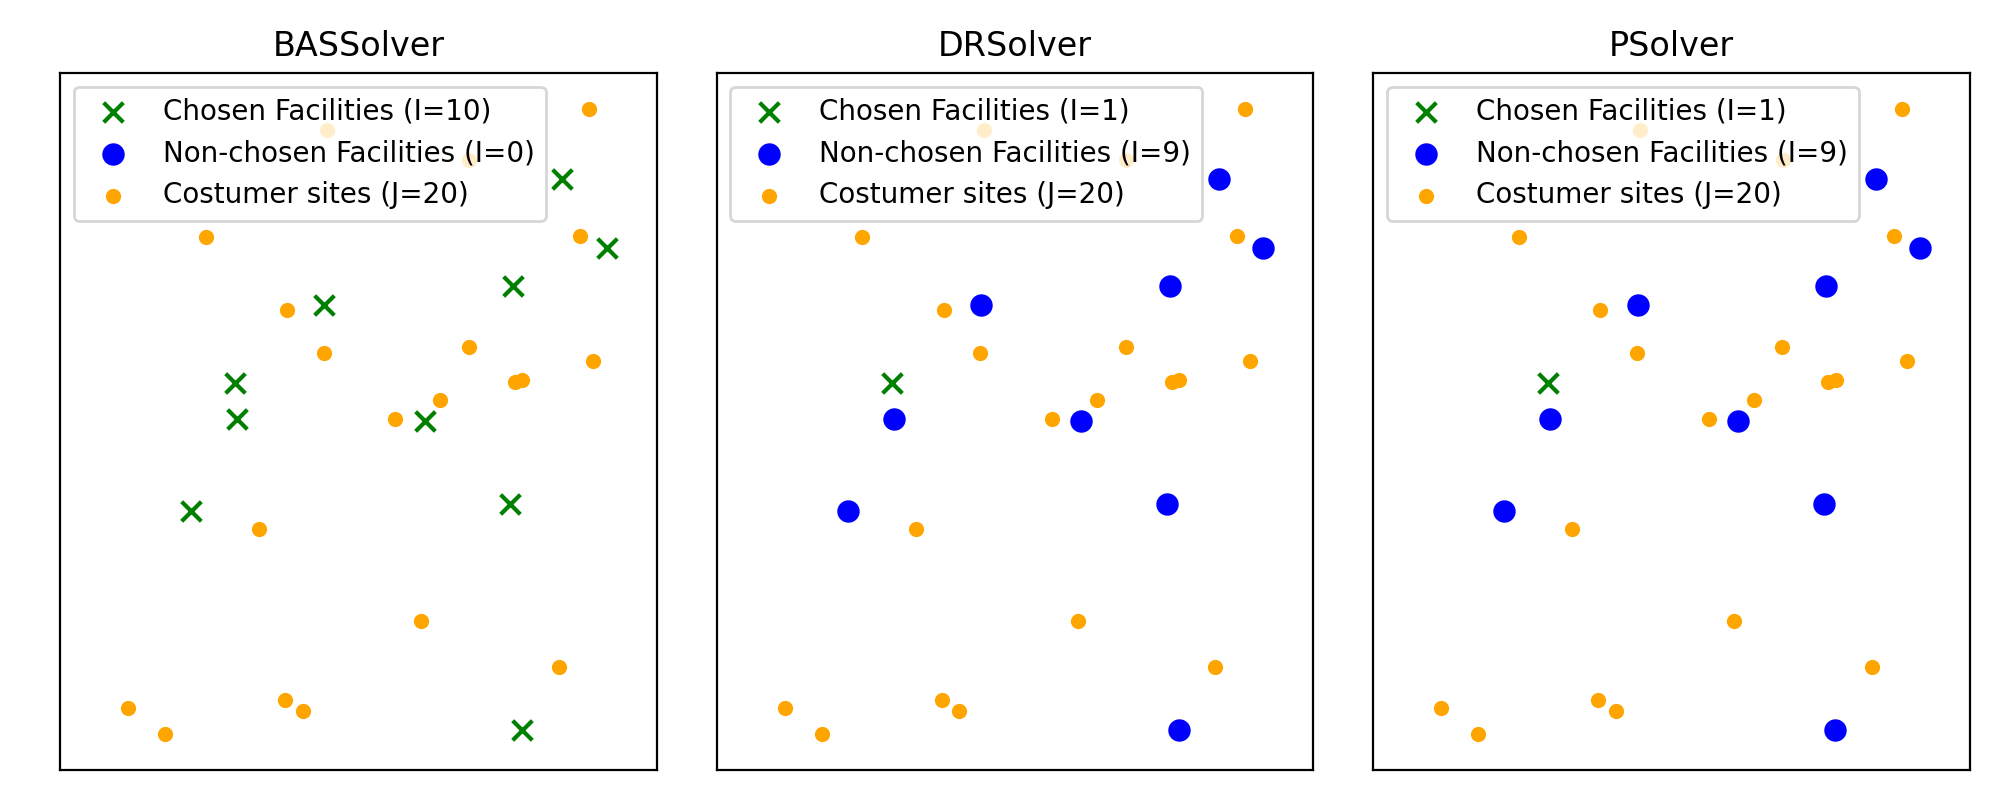
\includegraphics[width=\textwidth]{../figure/chosen_facility_costumer_site_pos.png}
		\caption{Optimal decision of different models}
		\label{fig:decisions}		
	\end{figure}
	
	Figure \ref{fig:comparison}, compares the optimal objective value of different models, and how many units of product, $s$, decision maker have to buy from a third party company and pay $p$ for each unit. We can see \gls{dddro}, has lowest total cost. The result, also algins with unsatisfied demand. This is because $p$ is a high penalty and model decides to open more facilities, and not pay high cost $p$.

	\begin{figure}[h!]
	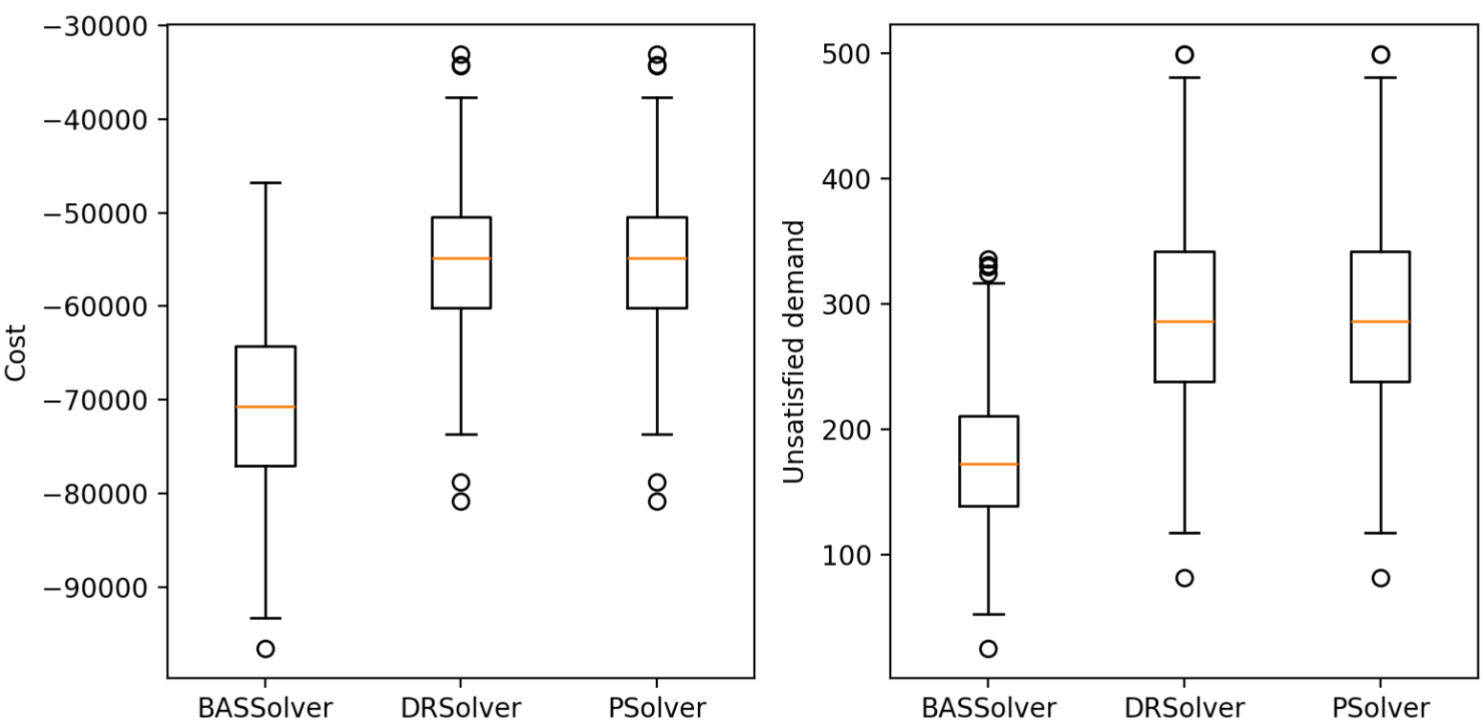
\includegraphics[width=\textwidth]{../figure/comparision.png}
	\caption{Comparison of the performance of different models}
		\label{fig:comparison}		
	\end{figure}

	\newpage
	\printglossary[type=\acronymtype]
	
	\clearpage
	\bibliography{../ref}
	\bibliographystyle{apalike}
\end{document}
